\documentclass{tikzposter} % See Section 3

\usepackage{natbib}
\usepackage{mciteplus}
\usepackage[T1]{fontenc}
\usepackage{fontspec}

\title{Retention Time Alignment}
\institute{University Medical Center, Johannes Gutenberg University, Germany}
\author{Mateusz Krzysztof Łącki, Ute Distler, Stefan Tenzer} %\titlegraphic{Logo}
\usetheme{Simple} % See Section 5
\usetitlestyle{Filled}


\begin{document}
\maketitle % See Section 4.
\block{Rationale}{
Modern LC-IM-MS devices can easiy identify thousands of peptides contained in the proteolitically digested analytes.
This knowledge is later used to infer the presence of proteins.
However, the majority of observed signals are not easily sequenced rendering them useless in the identification process.
As seen in Panel~A~in~Figure~\ref{fig:seq_vs_unseq}, the number of unsequenced signals can exceed the number of sequenced peptides tenfold.


\begin{tikzfigure}[Caption of the figure]
\label{fig:seq_vs_unseq}
	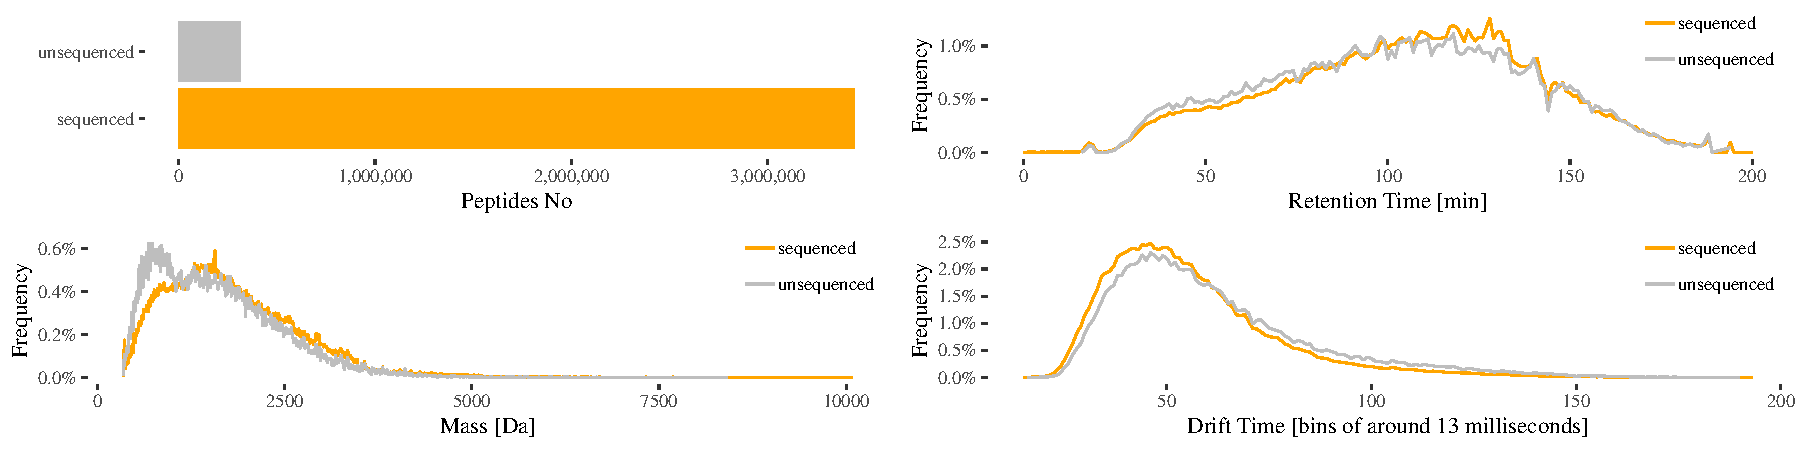
\includegraphics[width=\linewidth]{R/img/seq_vs_unseq_plot}
\end{tikzfigure}

} % See Section 4.2

\begin{columns} % See Section 4.4
\column{0.3} % See Section 4.4
\block{BlocktitleB}{Blocktext}
\column{0.7}
\block{BlocktitleC}{Blocktext}
\end{columns}

%\note{Notetext} % See Section 4.3
\end{document}
